
\chapter{集合}
\label{chap:set}

\section{文氏图}
\label{sec:venn-diagram}

\begin{example}
  一(4)班共有50人,其中28人有哥哥,26人有弟弟,15人没有兄弟。那么只有哥哥没有弟弟的有多少人?只有弟弟没有哥哥的有多少人?既有哥哥也有弟弟的有多少人?
\end{example}
\begin{proof}[提示]这种问题最适合用文氏图来解决。
  \begin{center}
    \begin{tikzpicture}[scale=1.0]
      \begin{scope}[blend mode=multiply]
        \draw(0,0)rectangle(4,3);
        \filldraw[fill=red!20,opacity=.5](1.5,1.5)circle(1);
        \filldraw[fill=blue!20,opacity=.5](2.5,1.5)circle(1);
        \draw[->](1,1.5)--(-.5,1.5)node[left]{有哥哥的};
        \draw[->](3,1.5)--(4.5,1.5)node[right]{有弟弟的};
        \draw[->](3.5,2.6)--(4,3.5)node[above]{没有兄弟的};
        \draw[->](2,1.5)--(0,3.5)node[above]{既有哥哥也有弟弟的};
      \end{scope}
    \end{tikzpicture}
  \end{center}
  如上图,用长方形表示整个班的人,左边的圆表示有哥哥的人,右边的圆表示有弟弟的人,两个圆相交的部分表示既有哥哥又有弟弟的人(如果班上没有既有哥哥也有弟弟的人,则两个圆不相交)。则左圆左边部分表示只有哥哥的人,右圆的右边部分表示只有弟弟的人,两圆外空白的部分表示没有兄弟的人。由此,可以先填入15。
  \begin{center}
    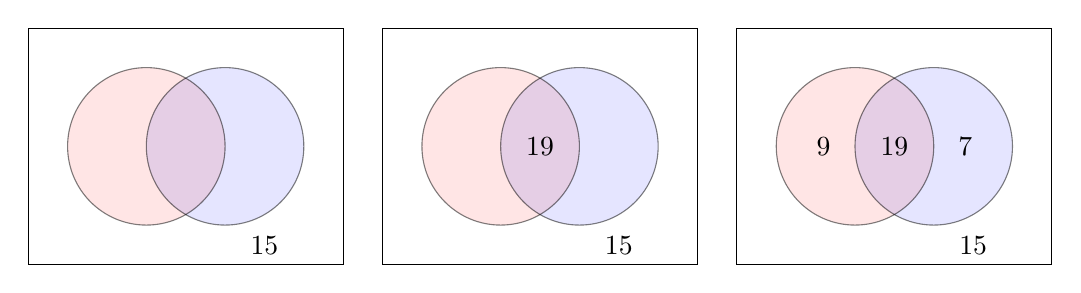
\begin{tikzpicture}[scale=1.0]
      \begin{scope}[blend mode=multiply]
        \draw(0,0)rectangle(4,3);
        \filldraw[fill=red!20,opacity=.5](1.5,1.5)circle(1);
        \filldraw[fill=blue!20,opacity=.5](2.5,1.5)circle(1);
        \node[above] at (3,0) {15};
      \end{scope}
      \begin{scope}[blend mode=multiply,shift={(4.5,0)}]
        \draw(0,0)rectangle(4,3);
        \filldraw[fill=red!20,opacity=.5](1.5,1.5)circle(1);
        \filldraw[fill=blue!20,opacity=.5](2.5,1.5)circle(1);
        \node[above] at (3,0) {15};
        \node at (2,1.5){19};
      \end{scope}
      \begin{scope}[blend mode=multiply,shift={(9,0)}]
        \draw(0,0)rectangle(4,3);
        \filldraw[fill=red!20,opacity=.5](1.5,1.5)circle(1);
        \filldraw[fill=blue!20,opacity=.5](2.5,1.5)circle(1);
        \node[above] at (3,0) {15};
        \node at (2,1.5){19};
        \node at (1.1,1.5){9};
        \node at (2.9,1.5){7};
      \end{scope}
    \end{tikzpicture}
  \end{center}
  两个圆加起来的部分共有$50-15=35$人,从而可以填入两圆共同的部分$28+26-35=19$人,只有哥哥的$28-19=9$人,只有弟弟的$26-19=7$人。
\end{proof}


\section{极坐标}
\label{sec:polar-coordinate}

\begin{example}[极坐标的魔法]\mbox{}\par
  \begin{center}
    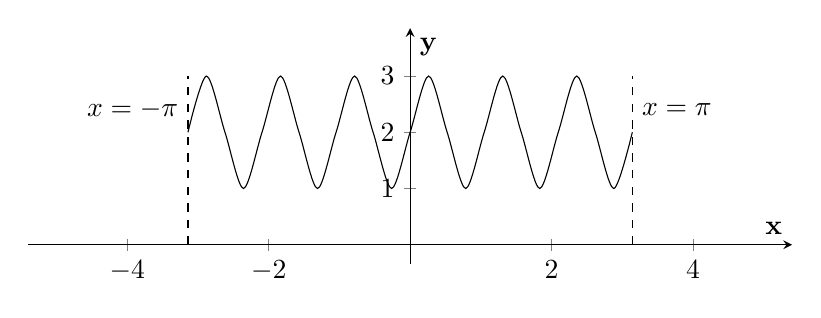
\begin{tikzpicture}[scale=1.0]
      % \draw[help lines](0,0)grid(4,3);
      \begin{axis}[anchor=origin,
      scale only axis,
      width=0.8\textwidth,
      height=3cm,
      xmin = -4.5,
      xmax = 4.5,
      ymin = 0,
      ymax = 3.5, 
      axis lines = middle,
      enlargelimits = true,
      xlabel = {$\mathbf{x}$},
      ylabel = {$\mathbf{y}$}% ,
      % yticklabels={,,},
      % xticklabels={,,}
      ]
      \coordinate (A) at (axis cs:40,6);
      \addplot[domain=-3.1415926:3.1415926,smooth] (\x, {sin(deg(6*\x)) + 2});
      \draw[dashed] (-3.1415926,0)--(-3.1415926,3)node[pos=.8,left]{$x=-\pi$};
      \draw[dashed] (3.1415926,0)--(3.1415926,3)node[pos=.8,right]{$x=\pi$};
    \end{axis}
    \end{tikzpicture}
  \end{center}
  上面曲线在直角坐标系下的函数表达式为
  \begin{align*}
    y = \sin(6x) + 2
  \end{align*}
  相像一下,把$x$轴以及$x=-\pi$和$x=\pi$两直线围成的区域弯成一个圆,会是什么样呢?即将上面的函数变为极坐标形式
  \begin{align*}
    r = \sin(6\theta) + 2
  \end{align*}
  \begin{center}
    \begin{tikzpicture}[scale=1.0]
      \begin{polaraxis}
        \addplot+[mark=none,domain=0:360,samples=600]{sin(6*x)+2};
      \end{polaraxis}
    \end{tikzpicture}
  \end{center}
  这就是极坐标的魔力。
\end{example}

\begin{example}
  考虑曲线
  \begin{align*}
    y = \sin(2x) \cos(2x)
  \end{align*}
  \begin{center}
    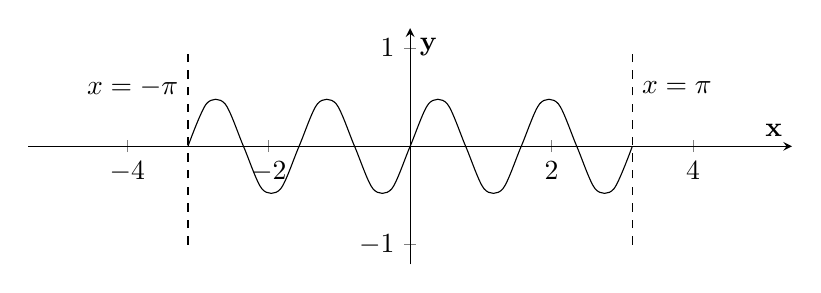
\begin{tikzpicture}[scale=1.0]
      % \draw[help lines](0,0)grid(4,3);
      \begin{axis}[anchor=origin,
      scale only axis,
      width=0.8\textwidth,
      height=3cm,
      xmin = -4.5,
      xmax = 4.5,
      ymin = -1,
      ymax = 1, 
      axis lines = middle,
      enlargelimits = true,
      xlabel = {$\mathbf{x}$},
      ylabel = {$\mathbf{y}$}% ,
      % yticklabels={,,},
      % xticklabels={,,}
      ]
      \coordinate (A) at (axis cs:40,6);
      \addplot[domain=-3.1415926:3.1415926,smooth] (\x, {sin(deg(2*\x)) * cos(deg(2*x))});
      \draw[dashed] (-3.1415926,-1)--(-3.1415926,1)node[pos=.8,left]{$x=-\pi$};
      \draw[dashed] (3.1415926,-1)--(3.1415926,1)node[pos=.8,right]{$x=\pi$};
    \end{axis}
    \end{tikzpicture}
  \end{center}
  弯成圆时,曲线变为
  \begin{align*}
    r = \sin(2\theta)\cos(2\theta)
  \end{align*}
    \begin{center}
    \begin{tikzpicture}[scale=1.0]
      \begin{polaraxis}
        \addplot+[mark=none,domain=0:360,samples=600]{sin(2*x)*cos(2*x)};
      \end{polaraxis}
    \end{tikzpicture}
  \end{center}
\end{example}